%
\section{Implementation}\label{sec:implementation}
This chapter explains how the component is developed. The ways to overcome the design challenges, some of the findings during the development have been written down.
%
\subsection{System Characteristics}
When beginning the implementation, I decided to use a simple yet powerful programming language for both frontend and backend applications to obtain my results. The programing languages which I selected was javascript for frontend and C\# for the backend. To simplify my programming work, I used the Visual Studio Code IDE for the frontend and Visual Studio 2019 for the backend. The configuration of the computer used for implementation is as follows:
\begin{description}
	\item [$\bullet$]Operating System: Windows 10 Enterprise 2016 - 64-bit
	\item [$\bullet$]Processor: Intel Core i7-6700 @ 3.4GHz
	\item [$\bullet$]RAM: 16GB
	\item [$\bullet$]HDD: 500GB
\end{description}

The software support tools used for frontend implementation are listed as follows:
\begin{description}
	\item [$\bullet$]Programming Language: Javascript
	\item [$\bullet$]IDE: Visual Studio Code
	\item [$\bullet$]Packet Manager: npm
	\item [$\bullet$]Version Control: Azure Repos
\end{description}

The software support tools used for backend implementation are listed as follows:
\begin{description}
	\item [$\bullet$]Programming Language: C\#
	\item [$\bullet$]IDE: Visual Studio 2019
	\item [$\bullet$]Packet Manager: NuGet
	\item [$\bullet$]Database: Azure Data Storage - Containers
	\item [$\bullet$]Version Control: Azure Repos
\end{description}

All the infrastructure and software that I used are provided by evosoft GmbH.
\subsection{OSS Component Analyzer}
The OSS component analyzer is a starting point in the process of scanning the OSS components from a project. This is a front-end module and it is implemented in the Angular framework using typescript language. The GUI interface of this module requires four inputs from the user which is project name, description, members and project source directory. It has two important tasks before it proceeds to the evaluation process. The first task, the module should find the required configuration file in the project. This configuration file identification was done with the help of a dependency manager. Each application framework has its own dependency manager and it generates a unique configuration file for the application framework. The below table shows all the config files of each application framework. The OSS component names and versions will be listed in the config files. 
\begin{table}[h!]
\begin{center}
 \begin{tabular}{ |c|c|c|c| } 
 	\hline
 	Application Framework & Dependency Manager & Config file & File Type \\
 	\hline
 	.NET(Console Application) & Nuget & .csproj file & XML \\ 
 	Angular Framework & npm & package.json & JSON \\ 
 	Microsoft TFS & Nuget & app.config & XML \\ 
 	Django & npm & requirremen.txt & Text\\ 
 	Ruby on Rails & Rubygem & gemfile & File \\ 
 	Laravel & composer & composer.json & JSON \\ 
 	Gradle projects & gradle & build.gradle & GRADLE \\ 
 	Maven projects & POM & pom.xml & XML \\ 
 	.NET & Nuget & packages.config & XML \\ 
 	\hline
 \end{tabular}
\caption{Configuration file of each application framework.}\label{tab:configFiles}
\end{center} 
\end{table}

Once the respective config is identified from the project, the targeted data should be scrapped from config files. To achieve this, the automated scrapping methods are used based on the config file type. For instance the user is scanning Maven project, then according to the table the config file is a XML file so therefore to scrap the targeted data DOM parsing method is used. Likewise for JSON file json parsing methods can be used, text pattern matching methods can be used for text file, Gemfile, FIle and GRADLE files.
\newpage
 \begin{figure}[h!]
	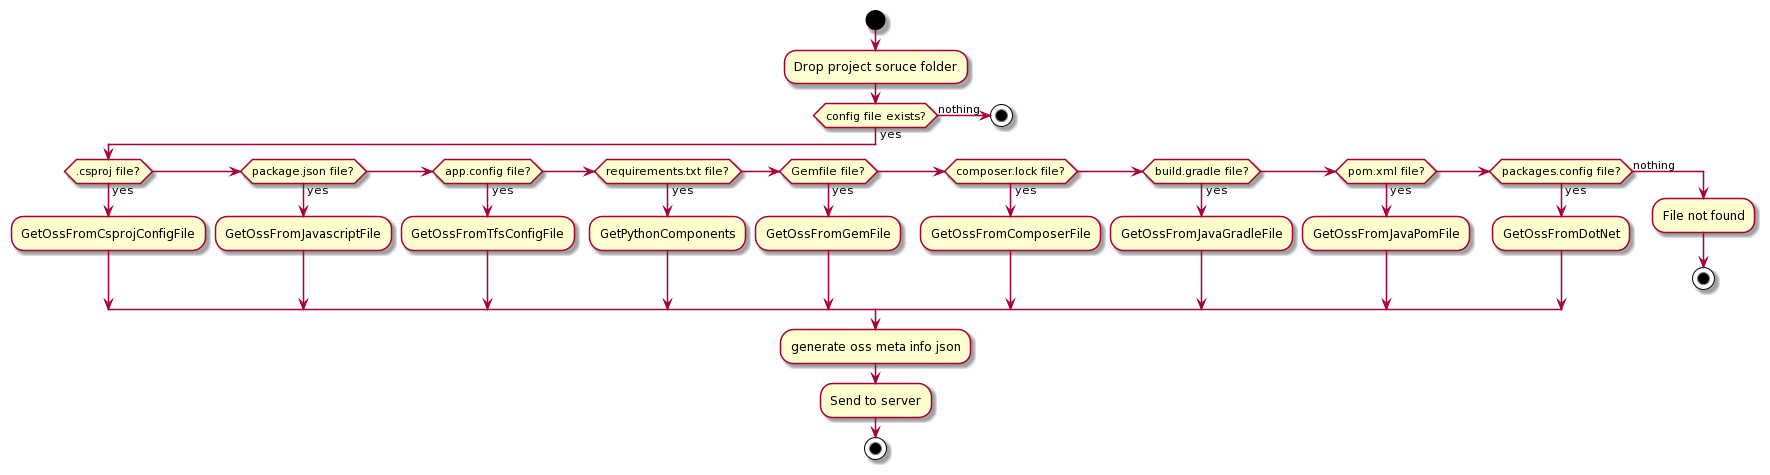
\includegraphics[width=15cm]{includes/OSS_Analyzer_Activity_Diagram.png}
	\centering
	\caption{\acs{OSS} scanner architecture}
	\label{fig:Analyzer_Activity_Diagram}
\end{figure}
\subsection{Component Evaluator}

\subsection{Reporter}
%
